\section{Uncertainty Dependency of $X$ and $P$}\label{sec:3}
Now we focus on how the uncertainty changes as a function of $X$ and $P$.
The $\pi$ values were calculated for 16 different combinations of point- and
experiment count. The results are shown in \cref{tab:ex1.5_pi_values} with
the corresponding histograms for the $\pi_x$ distributions.
It is easy to see that for a constant $P$ the uncertainty does not
change with higher $X$ which is surprising, because it means that for a
given number of generated points the $\pi$ value cannot be made
more precise with higher experiment count. The uncertainties for every
$P$ are shown in \cref{fig:uncertainty_function_of_x} where no particular 
correlation can be seen. In \cref{fig:uncertainty_function_of_p}
a correlation between the uncertainty and $P$ for constant $X$
is clearly visible. For the log-log plot in \cref{fig:uncertainty_function_of_p} a linear
function would be a good approximation, thus we can write
$$ \log \text{err}(P) = -n\log P + b$$
with $b, n > 0$. This results in the relation
$$\text{err}(P) = \frac{\mathrm{e}^b}{P^n}$$
for the uncertainty. This function will not be fitted to the data but from visual
inspection it is clear that the same relation with same parameters $b$ and $n$
will hold for every $X$. \par
With this information we can conclude that the most efficient way to calculate
$\pi$ with a given $PX$ is to maximize $P$ and keep $X$ small, although From
\cref{sec:1} it is known that $X$ has to be atleast bigger than $1$.
%
%$X \text\textbackslash P$ & 10 & 100 & 1000 & 10000 
\begin{table}
\centering
\caption{
    Calcuated $\pi$ values for different $P$ and $X$.
    }
\label{tab:ex1.5_pi_values}
\begin{tabular}{c|cccc}
\toprule
P & 10 & 100 & 1000 & 10000 \\
X &  &  &  &  \\
\midrule
10 & \num{3.16 \pm 0.488} & \num{3.208 \pm 0.156} & \num{3.156 \pm 0.046} & \num{3.144 \pm 0.018} \\
100 & \num{3.1 \pm 0.608} & \num{3.138 \pm 0.161} & \num{3.139 \pm 0.055} & \num{3.142 \pm 0.016} \\
1000 & \num{3.135 \pm 0.519} & \num{3.143 \pm 0.16} & \num{3.142 \pm 0.052} & \num{3.141 \pm 0.016} \\
10000 & \num{3.134 \pm 0.518} & \num{3.14 \pm 0.164} & \num{3.141 \pm 0.052} & \num{3.142 \pm 0.016} \\
\bottomrule
\end{tabular}
\end{table}

%
\begin{figure}[htbp]
	\centering
	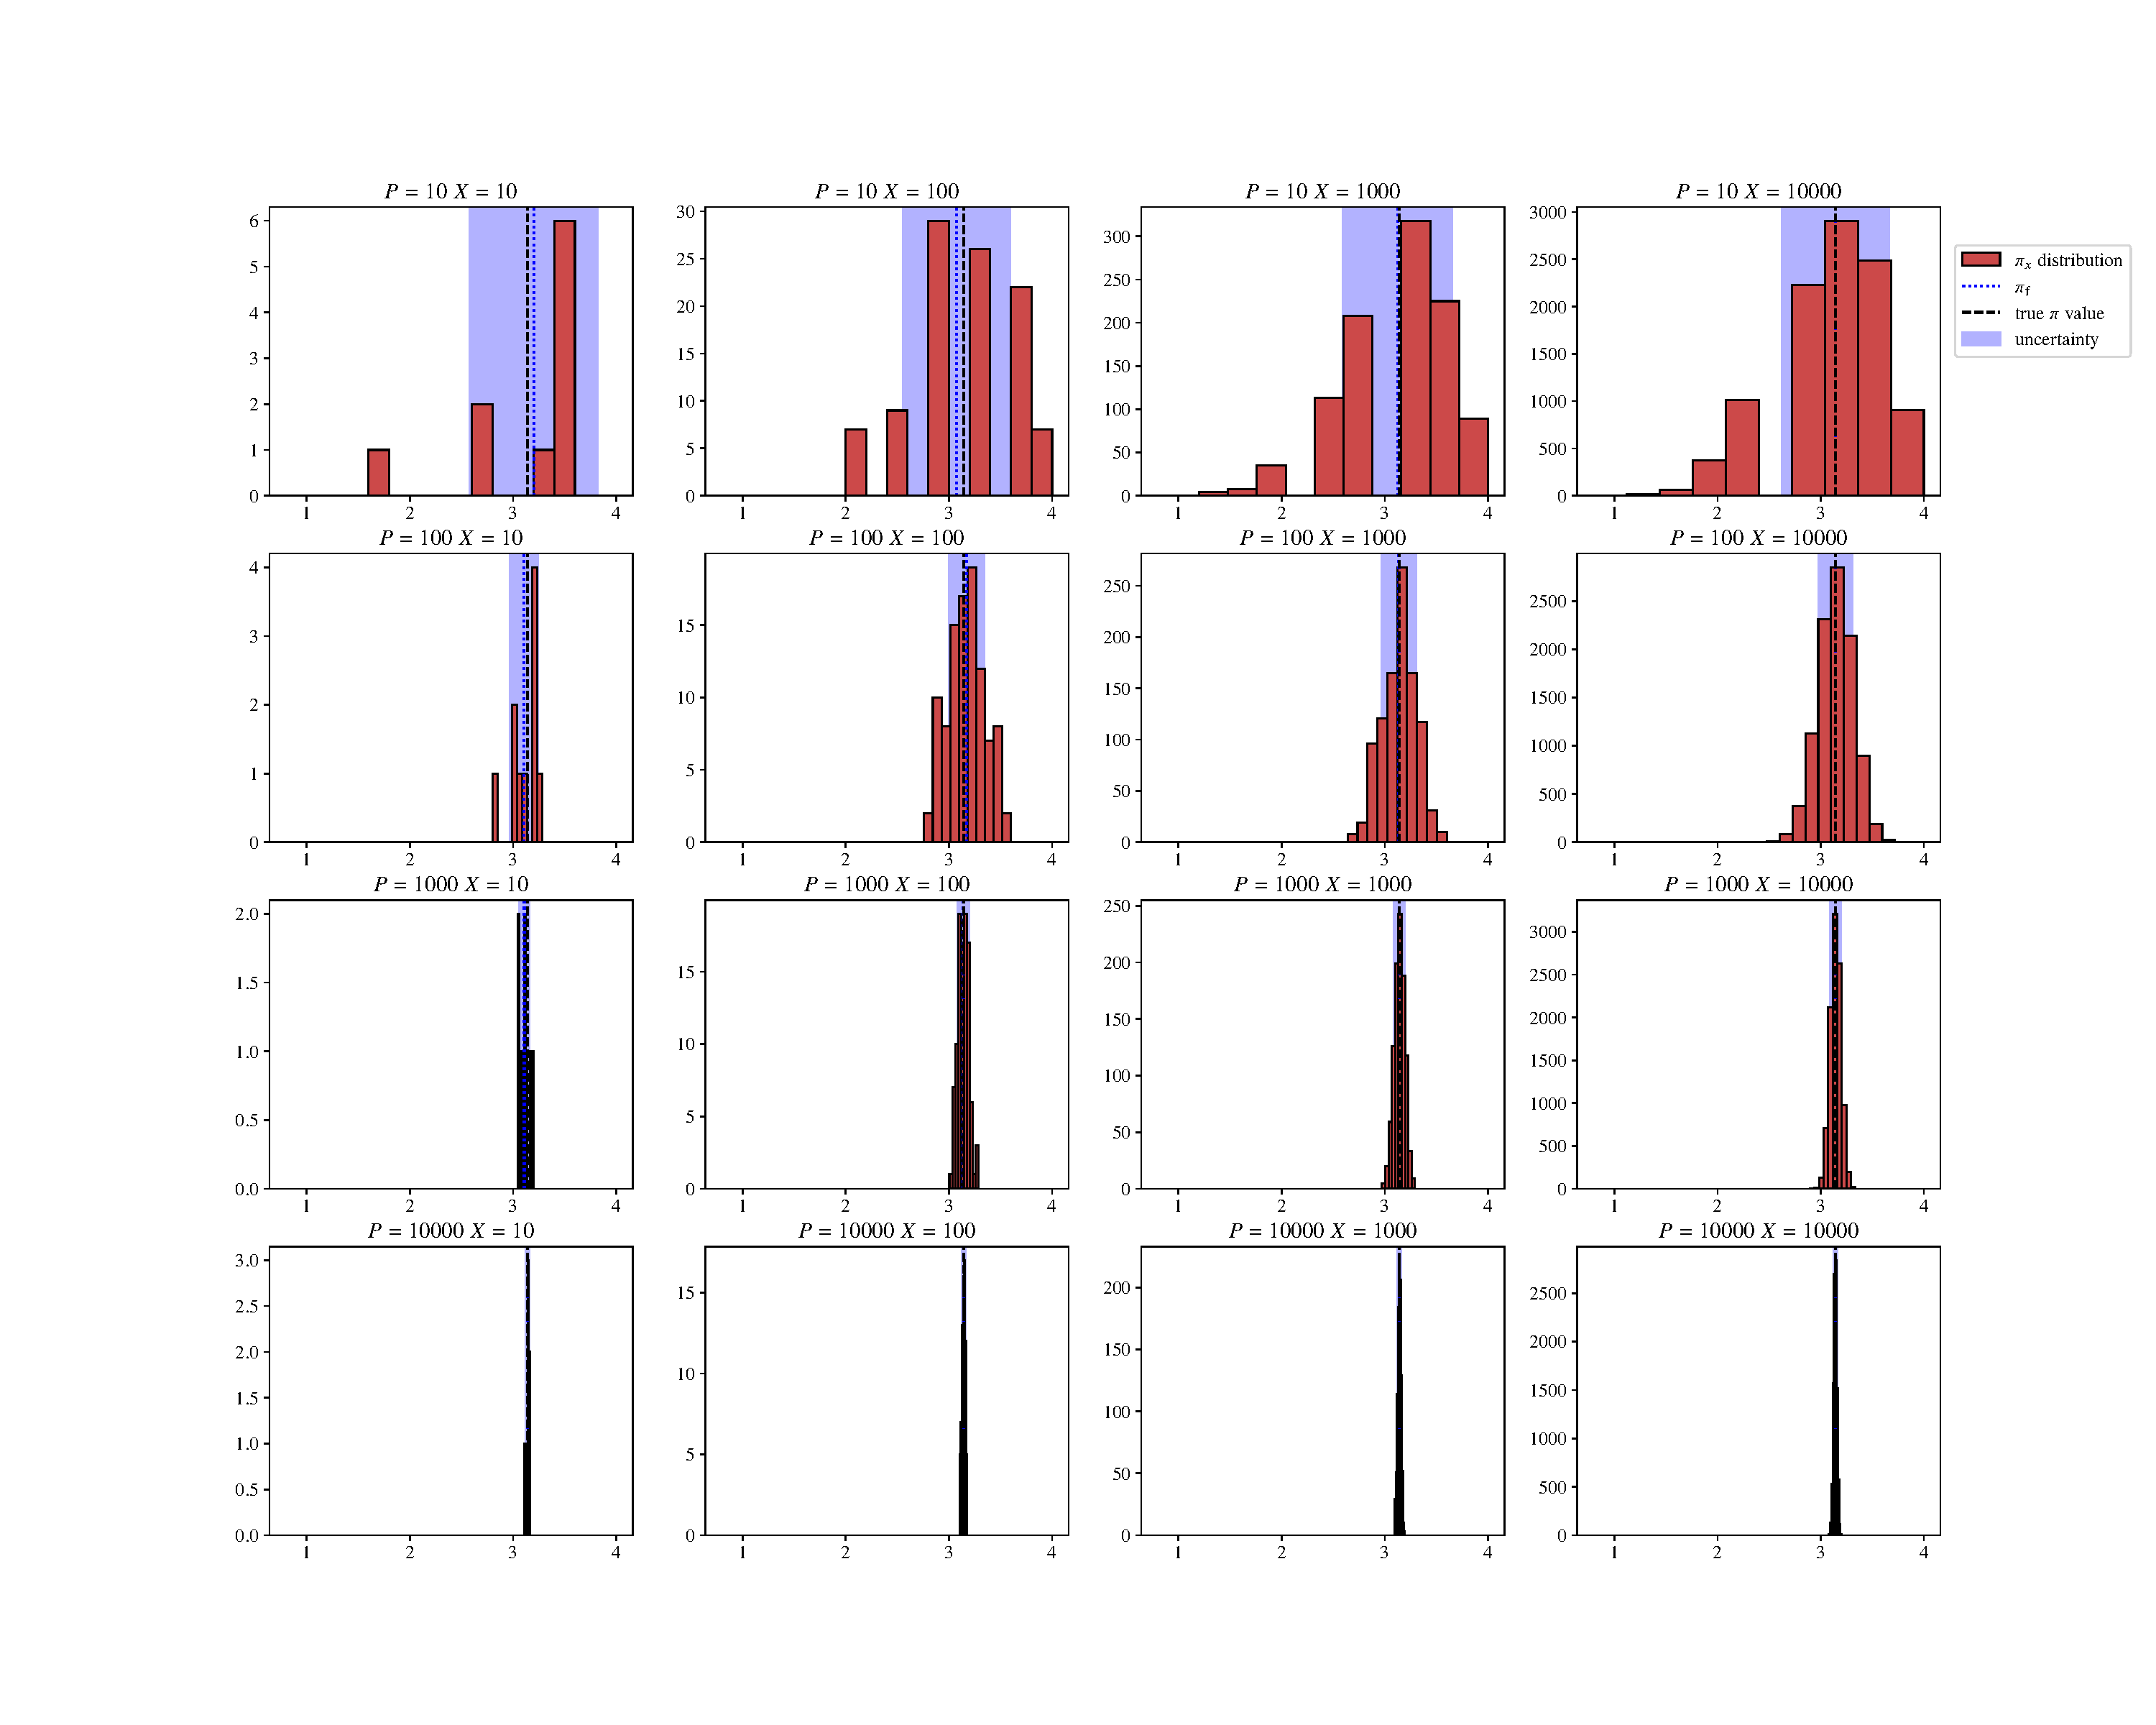
\includegraphics[width=1\linewidth]{figs/ex1.5_px_combinations.pdf}
	\caption{$\pi_x$ distributions for different combinations of $P$ and $X$.}
	\label{fig:px_combinations}
\end{figure}
%
\begin{figure}[htbp]
	\centering
	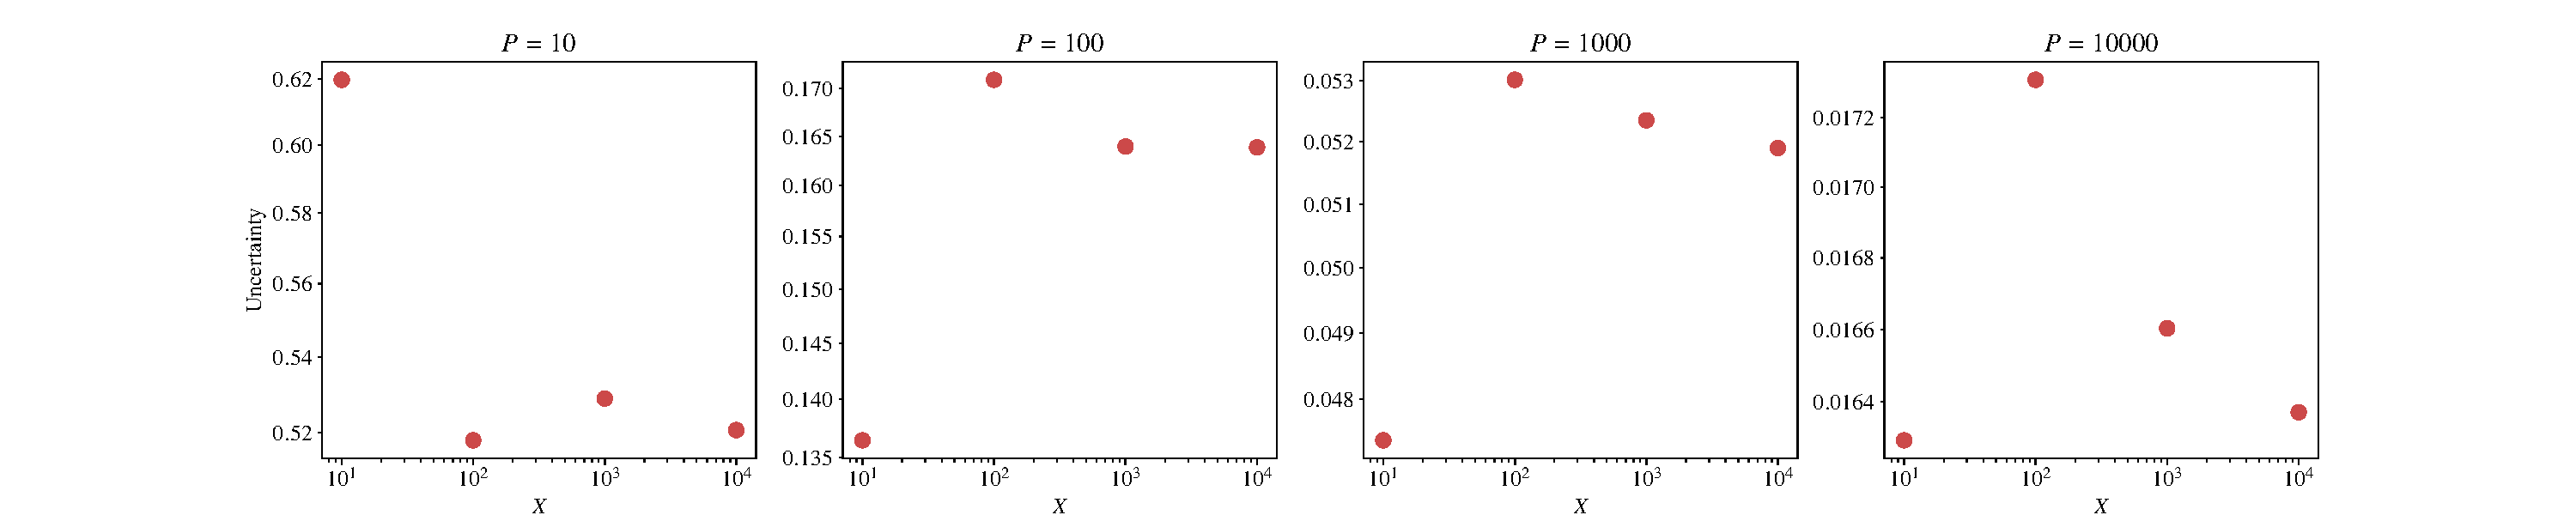
\includegraphics[width=\linewidth]{figs/1.5_uncertainty_function_of_x.pdf}
	\caption{Uncertainty as a function of $X$ for different $P$ values.}
	\label{fig:uncertainty_function_of_x}
\end{figure}
%
\begin{figure}[htbp]
	\centering
	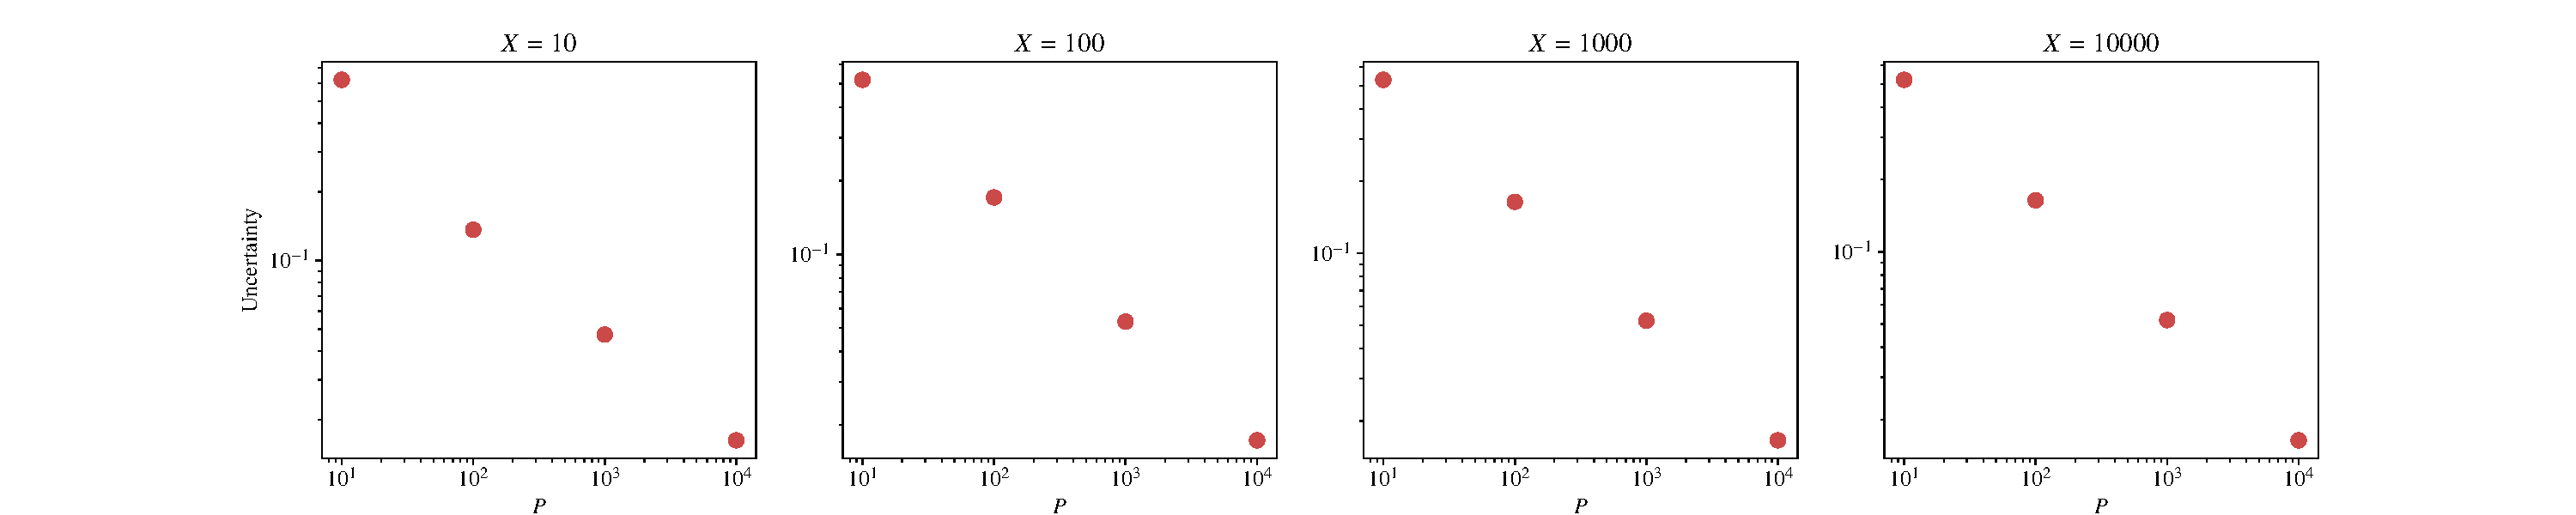
\includegraphics[width=\linewidth]{figs/1.5_uncertainty_function_of_p.pdf}
	\caption{Uncertainty as a function of $P$ for different $X$ values.}
	\label{fig:uncertainty_function_of_p}
\end{figure}